\documentclass[12pt,letterpaper]{article}
\usepackage[utf8]{inputenc}
\usepackage[spanish]{babel}
\usepackage{graphicx}
\usepackage[left=2cm,right=2cm,top=2cm,bottom=2cm]{geometry}
\usepackage{graphicx} % figuras
% \usepackage{subfigure} % subfiguras
\usepackage{float} % para usar [H]
\usepackage{amsmath}
%\usepackage{txfonts}
\usepackage{stackrel} 
\usepackage{multirow}
\usepackage{enumerate} % enumerados
\renewcommand{\labelitemi}{$-$}
\renewcommand{\labelitemii}{$\cdot$}
% \author{}
% \title{Caratula}
\begin{document}

% Fancy Header and Footer
% \usepackage{fancyhdr}
% \pagestyle{fancy}
% \cfoot{}
% \rfoot{\thepage}
%

% \usepackage[hidelinks]{hyperref} % CREA HYPERVINCULOS EN INDICE

% \author{}
\title{Caratula}

\begin{titlepage}
\begin{center}
\large{UNIVERSIDAD PRIVADA DE TACNA}\\
\vspace*{-0.025in}
\begin{figure}[htb]
\begin{center}

\includegraphics[width=7cm]{./images/logo}
\end{center}
\end{figure}
\vspace*{0.15in}
INGENIERIA DE SISTEMAS  \\

\vspace*{0.3in}
\begin{large}
\textbf{TITULO:} \\
\end{large}

\vspace*{0.1in}
\begin{Large}
\textbf{Informe de Laboratorio 04 Crear una Dimensión Regular con SQL Server Analysis Services} \\

\end{Large}

\vspace*{0.3in}
\begin{Large}
\textbf{CURSO:} \\
\end{Large}

\vspace*{0.1in}
\begin{large}
INTELIGENCIA DE NEGOCIOS\\
\end{large}

\vspace*{0.3in}
\begin{Large}
\textbf{DOCENTE:} \\
\end{Large}

\vspace*{0.1in}
\begin{large}
 Ing. Patrick Cuadros Quiroga\\
\end{large}

\vspace*{0.4in}
\vspace*{0.1in}
\begin{large}
\textbf{INTEGRANTES:} \\
\begin{flushleft}
Willian Huillca Umpiri \hfill	(2015053793)\\

\centering  %CENTRA UN TEXTO
\vspace*{0.9in}
\begin{large}
TACNA-PERU
\end{large}

\end{flushleft}
\end{large}
\end{center}

\end{titlepage}


\tableofcontents % INDICE
\thispagestyle{empty} % INDICE SIN NUMERO
\newpage
\setcounter{page}{1} % REINICIAR CONTADOR DE PAGINAS DESPUES DEL INDICE


\section{Procedimientos}

Tomando como base el laboratorio anterior se construyo un cubo básico Multidimensional, pero se tenia dificultad al momento de explotar la información. Este detalle se debe a que no tuvimos un manejo más personalizado de los atributos de las dimensiones. En este laboratorio se abordará como crear y configurar una dimensión regular en Analysis Services.
\begin{center}
\end{center}

\section{EJERCICIO 01: Creación de una Dimensión Regular} 

\textbf{}\\\\
En el Solution Explorer nos ubicamos en Data Sources View y podemos ver que tenemos la vista de las siguientes tablas:
\begin{center}
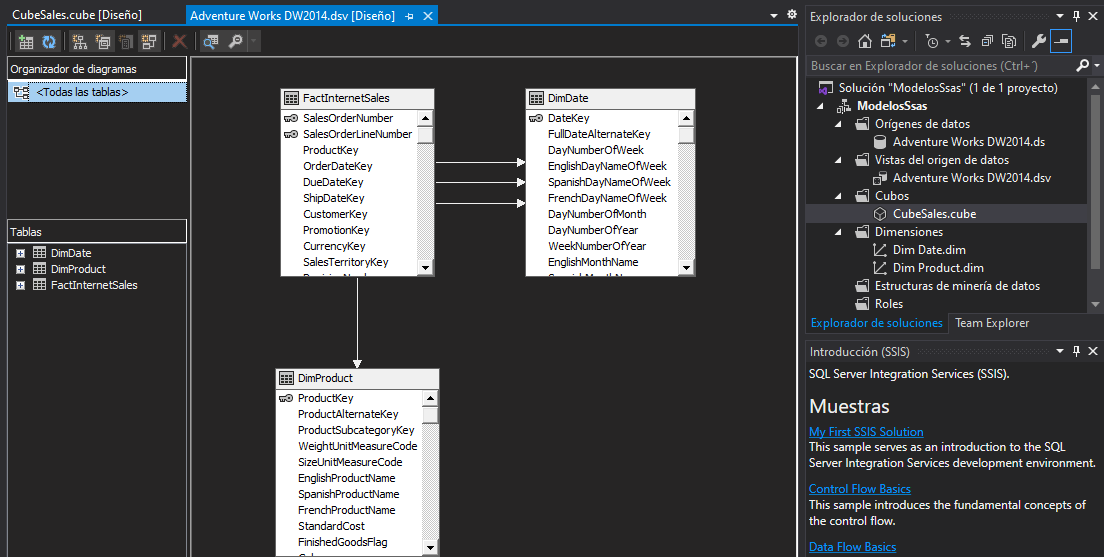
\includegraphics[width=\columnwidth]{images/task1/1}\newline
\end{center}

Nos abrirá un Wizard, donde la primera ventana es un resumen de lo que se puede realizar.
\begin{center}
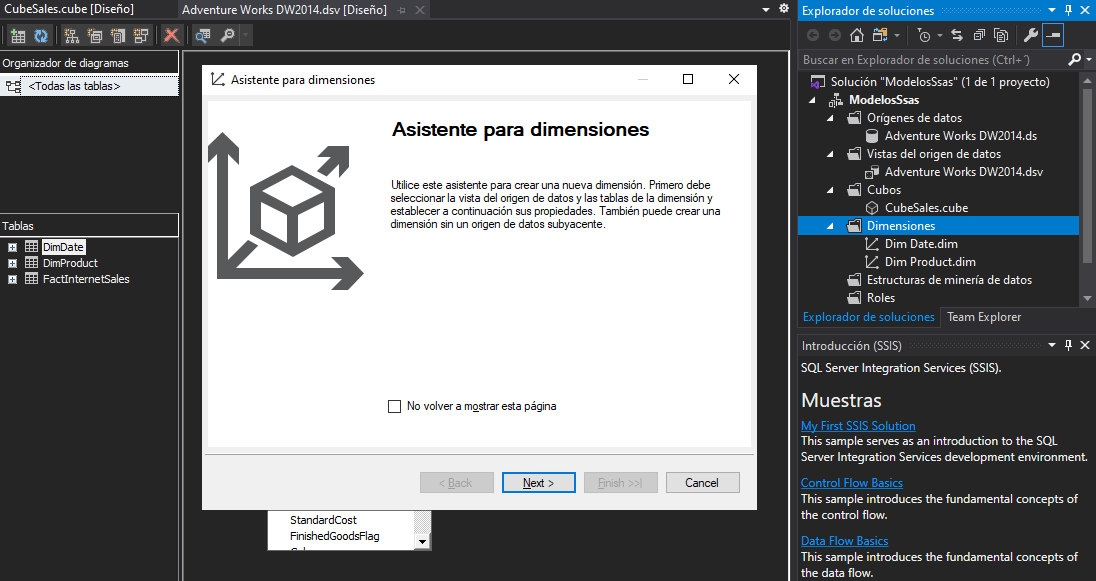
\includegraphics[width=\columnwidth]{images/task1/2}\newline
\end{center}



Esta paso en el wizard es muy importante ya que nos permite seleccionar el origen de la dimensión a crear. 
Seleccionamos la primera opción:
\begin{center}
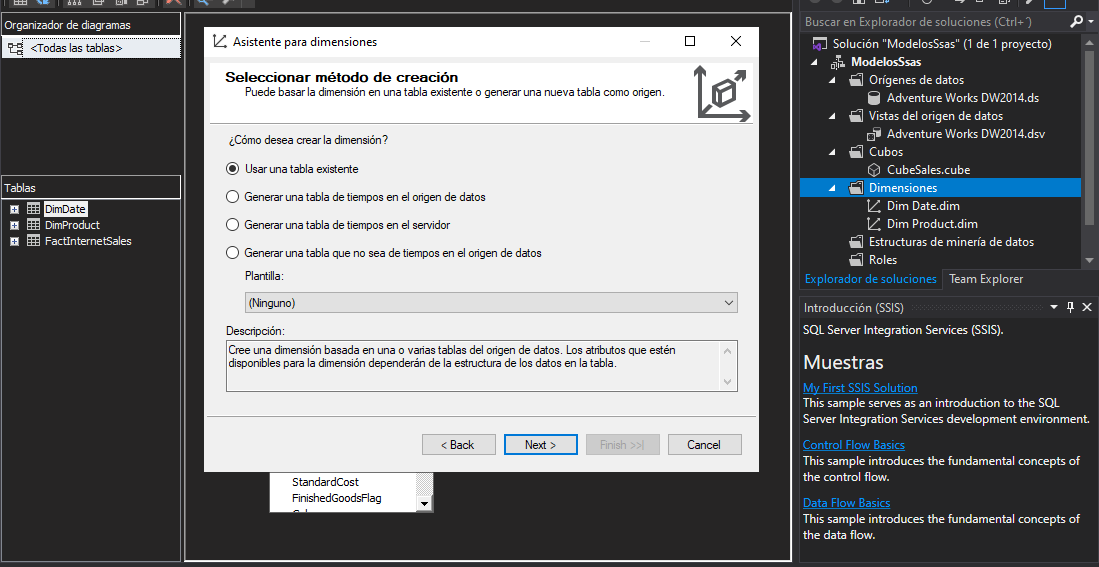
\includegraphics[width=\columnwidth]{images/task1/3}\newline
\end{center}

Seleccionamos el Data source view (podríamos tener más de uno) y la tabla Dimensión, en este ejemplo DimProduct. En Key columns por defecto siempre selecciona al Primary Key de la tabla, pero este valor luego podría ser cambiado. También podemos añadirle un Name Column a este Key column pero lo dejaremos tal como esta:
\begin{center}
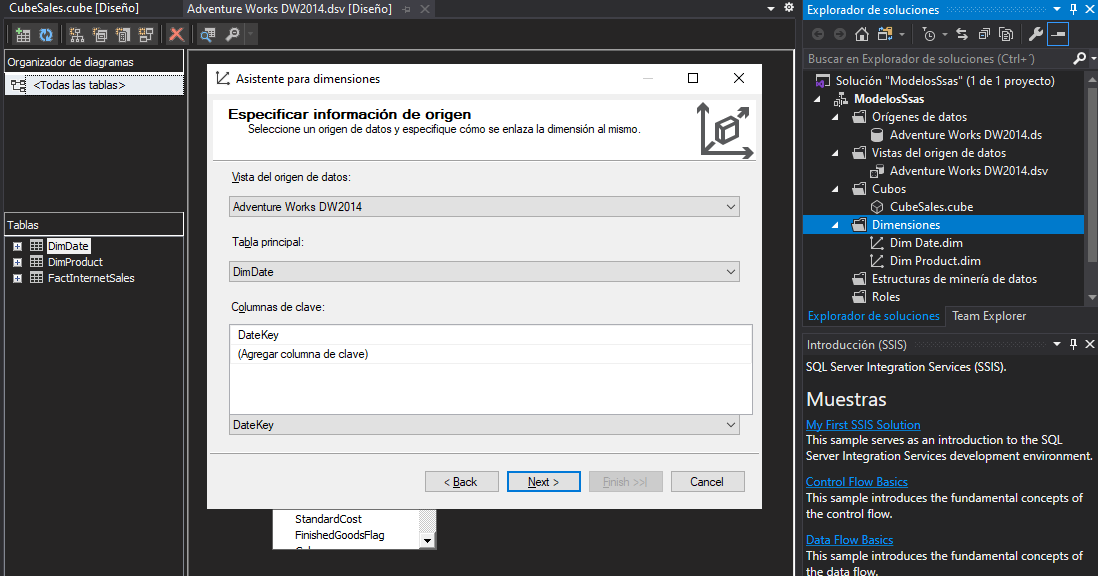
\includegraphics[width=\columnwidth]{images/task1/4}\newline
\end{center}

Marcamos los atributos con los cuales trabajaremos:
\begin{center}
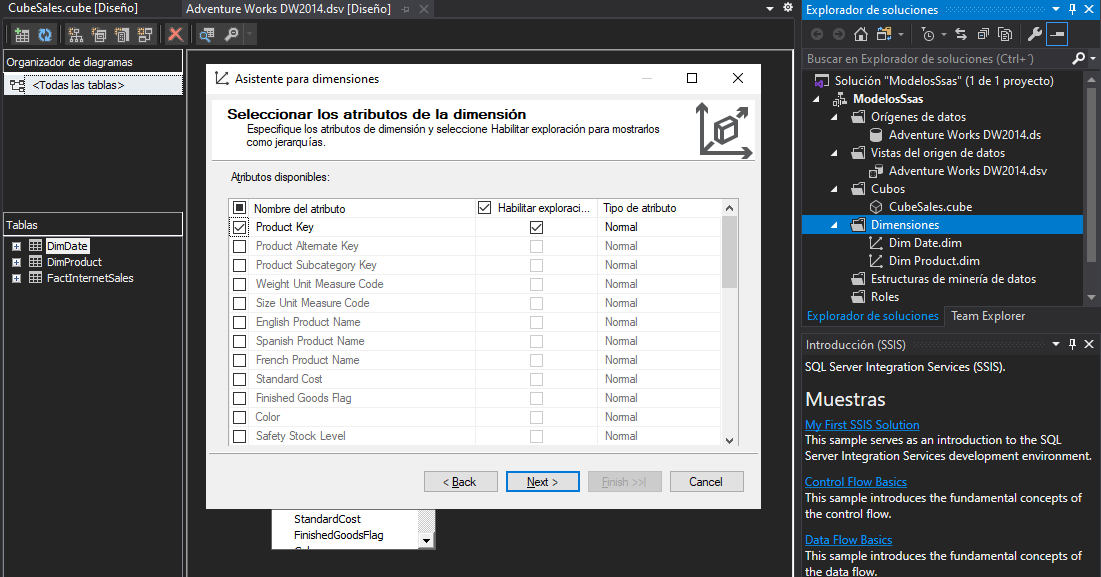
\includegraphics[width=\columnwidth]{images/task1/5}\newline
\end{center}

Indicamos el Nombre a la dimensión:
\begin{center}
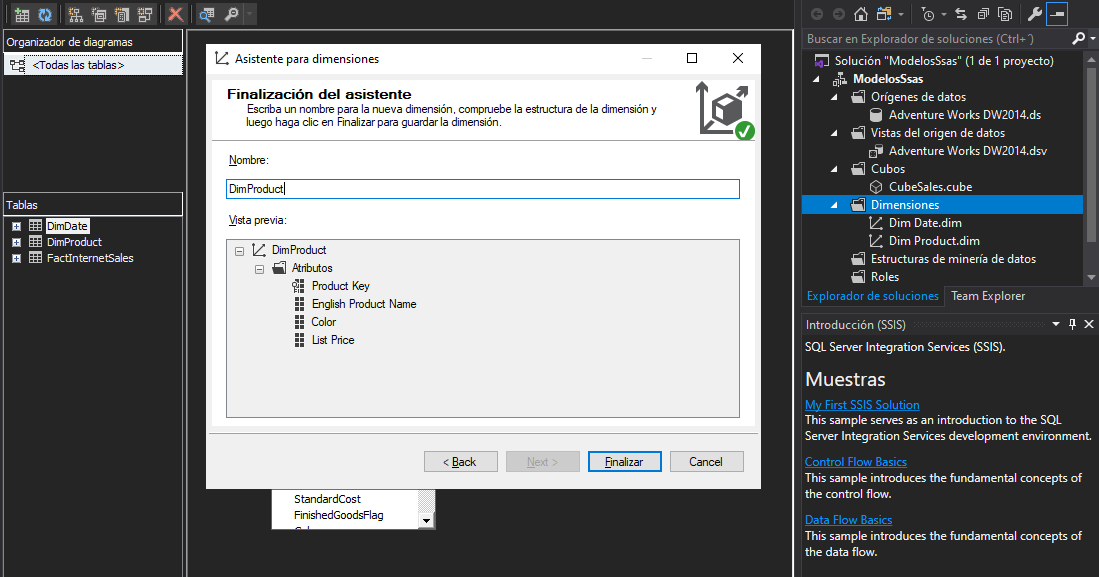
\includegraphics[width=\columnwidth]{images/task1/6}\newline
\end{center}


\section{EJERCICIO 02: Procesar una Dimensión} 

Ya creada la dimensión, el siguiente paso es Procesarla para ver la generación de los datos. En la pestaña de Dimension Structure ubicamos la opción de Process:
\begin{center}
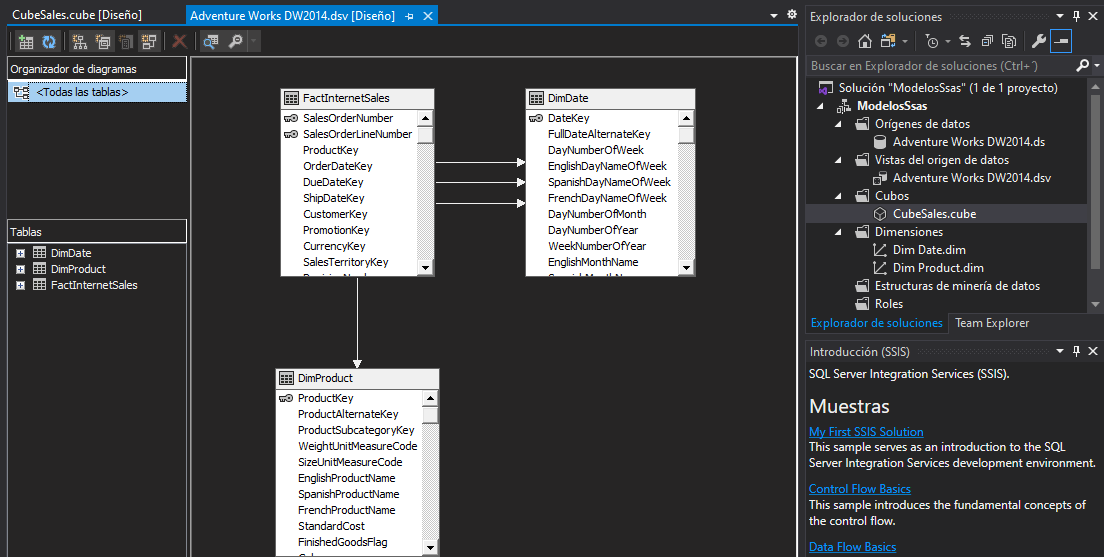
\includegraphics[width=\columnwidth]{images/task1/1}\newline
\end{center}


Es aquí donde detectamos que si bien es cierto nos muestra los valores de Product Key , lo recomendable es que este atributo no sea visible para el usuario final, ya que esta es una llave propia del DW
\begin{center}
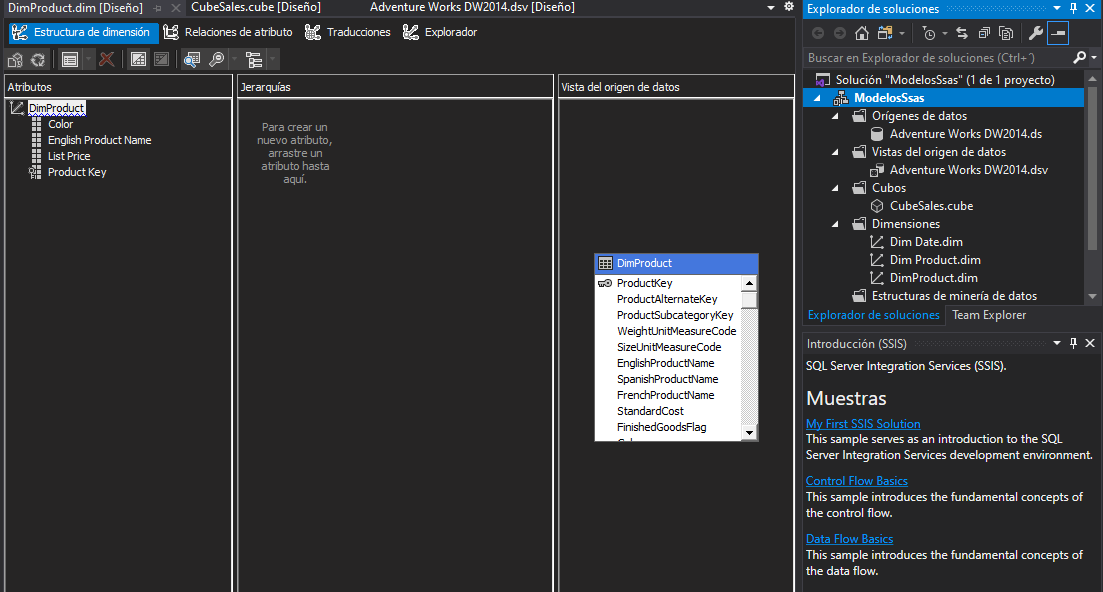
\includegraphics[width=\columnwidth]{images/task1/7}\newline
\end{center}


\section{*}


\section{*}



\end{document}